%
%                       This is a basic LaTeX Template
%                       for the Informatics Research Review

\documentclass[a4paper,11pt]{article}
% Add local fullpage and head macros
\usepackage{head,fullpage}     
% Add graphicx package with pdf flag (must use pdflatex)
\usepackage[pdftex]{graphicx}  
% Better support for URLs
\usepackage{url}
% Date formating
\usepackage{datetime}

\newdateformat{monthyeardate}{%
  \monthname[\THEMONTH] \THEYEAR}

\parindent=0pt          %  Switch off indent of paragraphs 
\parskip=5pt            %  Put 5pt between each paragraph  
\Urlmuskip=0mu plus 1mu %  Better line breaks for URLs


%                       This section generates a title page
%                       Edit only the following three lines
%                       providing your exam number, 
%                       the general field of study you are considering
%                       for your review, and name of IRR tutor

\newcommand{\examnumber}{B240710}
\newcommand{\field}{Network Science Analysis : An Elixir to Prevent Global Financial Crisis?}
\newcommand{\supervisor}{Xinran Ruan}

\begin{document}
\begin{minipage}[b]{110mm}
        {\Huge\bf School of Informatics
        \vspace*{17mm}}
\end{minipage}
\hfill
\begin{minipage}[t]{40mm}               
        \makebox[40mm]{
        \includegraphics[width=40mm]{crest.png}}
\end{minipage}
\par\noindent
    % Centre Title, and name
\vspace*{2cm}
\begin{center}
        \Large\bf Informatics Research Review \\
        \Large\bf \field
\end{center}
\vspace*{1.5cm}
\begin{center}
        \bf \examnumber\\
        \monthyeardate\today
\end{center}
\vspace*{5mm}

%
%                       Insert your abstract HERE
%                       
\begin{abstract}
The emerging global financial system marked a new era where institutions, markets, and players are interconnected and depending on each other. Although it boosts global economic progress, it is exposed to systemic risk due to its properties. Network science is then proposed to manage such risk because its properties resemble real-world global financial systems. In this review, we explore the multiple usages of network science in global stock markets and draw context of usage, advantages, and disadvantages for each of the methods for future use cases.
\end{abstract}

\vspace*{1cm}

\vspace*{3cm}
Date: \today

\vfill
{\bf Supervisor:} \supervisor
\newpage

%                                               Through page and setup 
%                                               fancy headings
\setcounter{page}{1}                            % Set page number to 1
\footruleheight{1pt}
\headruleheight{1pt}
\lfoot{\small School of Informatics}
\lhead{Informatics Research Review}
\rhead{- \thepage}
\cfoot{}
\rfoot{Date: \date{\today}}
%

\section{Introduction}
In the modern world, the global financial system is the intricate web of institutions, markets, and mechanisms that facilitates the flow of capital, currencies, and financial instruments on a worldwide scale. As the backbone of the modern global economy, this system connects individuals, businesses, governments, and financial entities across the world, forming a complex network of interactions among them. This network is instrumental for the aforementioned parties in allocating resources, managing risks, and supporting economic growth on international scale. Over the years, the network evolves following historical developments, technological advancements, and the dynamic nature of financial markets across the globe. Because of the interconnectedness properties of the network, it has emerged as a key driver of economic progress and a facilitator of cross-border collaborations.

However, despite the positive aspects that the global financial system offers to the world, it possesses an underlying risk that is able to collapse the international economy swiftly. The interdependencies properties of the network can transform a tiny disruption in one of the financial institutions inside the system into widespread or even total failure through cascading effect. This phenomenon is called systemic risk. The amplifying consequences of this risk is usually triggered by a shock or a series of interconnected events and often lead to global financial crisis.

Covid-19 pandemic is one of the recent examples of systemic risk effects in the global financial system. The first case of Covid was identified in China in December 2019, subsequently spreading to East Asia, Europe, and North America shortly after resulting in pessimism in the market. A significant turning point occurred on February 24, 2020, when the American stock market experienced a drastic decrease as indicated in both Dow Jones index and S\&P 500 index. The trend continued and hit the rock bottom on March 9 in which S\&P 500 index witnessed a 7\% dip and triggered a highly unusual stage 1 circuit breaker. It halted the stock market indefinitely to avoid the index plummeting even more. This created panic in the global markets, resulting in major indexes such as the FTSE 100, Frankfurt DAX 100, and Paris CAC 40 all decreasing subsequently, with the Sao Paulo B3 index receiving the hardest hit of -12.16\%. This collective downturn resulted in a global financial crisis in only a matter of 3 months. Within that timespan, the global gross domestic product (GDP) experienced a 3.4 \% decline, leading to a loss of economic output exceeding two trillion U.S. dollars. Considering the massive economic loss of the crisis, identifying the systemic risk in the financial systems as soon as possible is crucial to mitigate or lessen the impact of the global financial crisis.

As previously mentioned, the global financial system takes the form of a network and the systemic risk of such a network can be analyzed by examining its robustness and interaction behaviors through network science. Network science has emerged as a powerful tool for identifying and understanding systemic risk within interconnected systems, as it provides a framework to model, analyze, and visualize the relationships among units within that shape. In the network science field of study there is a terminology called contagion and it offers insights into how disruptions in one part of the network can propagate, leading to systemic implications that extend far beyond individual components. This allows for the identification of critical nodes, vulnerable pathways, and potential cascading effects. Researchers from around the globe have utilized network attributes to do systemic risk analysis from multiple angles. In this review, we will only focus on academic work due to its unbiased and transparent nature without disregarding companies, banks, and countries' contributions towards the utilization of network science in financial systems.

The potential of network science to do comprehensive analysis of systemic risk in financial networks raises important questions.
\begin{enumerate}
    \item To what extent can network science be employed as a tool for analyzing systemic risk in the global financial system and mitigate global crisis? 
    \item And what methodologies does network science offer in order to do the analysis? 
\end{enumerate}
The aim of this review is to answer those questions and showcase current network science methodologies that can be used to evaluate systemic risks in the global financial system, enhancing resilience and contributing to the overall stability of the system. 

The review does not assume knowledge of network science, therefore in section 2 we will include essential theoretical aspects of network science in order to familiarize readers with fundamental knowledge of the topic and solutions that are proposed. Some financial theories that act as foundation for the network science approaches will be included in each of the corresponding sections to avoid confusion and misunderstanding. However, we will not cover any in-depth financial calculation and theories in this review as we will focus more on the utilization of network science to mitigate the financial crisis.

Furthermore, we will examine three main approaches of network science that are mainly leveraged for that purpose in section 3. 
\begin{enumerate}
        \item Centrality measurement approach. This approach will identify important nodes within the network that play pivotal roles in the transmission of risks
        \item Connectivity approach. This approach will pinpoint things that influence the speed and extent of risk transmission
        \item Community detection approach. This approach will identify risk spread characteristics
\end{enumerate}

Conclusions and comments related to the topic will be presented in Section 4, while the final Section will highlight possible future research regarding the same topic.

In this research review, we will only focus on the financial system of the stock market and banks around the globe. Any other financial markets and instruments are not relevant in this review because each financial market will have its own attributes that contribute to different usage of network science. Additionally, we will only focus on the 2020 covid recession as it is the most up to date financial crisis and already covers multiple angles of network science approaches.

We base this review on peer-reviewed journals, articles, and also books to ensure the credibility of this review. We also limit the literature to be not older than 2011 as it is the initial usage of network science for systemic risk analysis in financial markets. Additionally, we also enrich the stated facts in this review using credible websites such as Investopedia and Statista.


\section{Network Science}
As the main topic of this research review, readers need to understand the fundamental concept of network science. It is critical for readers to connect the concept to further conceive the reasonings behind methodologies examined in this review. In this section, we will describe what network science actually is and several attributes that are substantial for systemic risk analysis.

\subsection{Definition}
Network science is a multidisciplinary field that explores the structure and dynamics of complex systems represented as networks. A network, in this context, is a representation of a real world system that consists of nodes connected by edges. These connections can represent a diverse range of relationships, from social interactions to the flow of information and structure of the system. Due to the variety of interactions, each edge can have direction and also weight that indicates the magnitude of interaction between nodes. This interdisciplinary approach draws on principles from mathematics, computer science, physics, sociology, and other fields to unravel the intricate patterns that underlie various systems.

One fundamental aspect of network science is the study of network topology, which refers to the arrangement and connectivity of nodes and edges within a network. By analyzing the topology, we gain insights into the emergent properties and behaviors of the system as a whole. This field has applications in diverse domains, including the financial system. Network science not only provides tools to describe the structure of these networks but also offers a framework to understand their evolution over time and the dynamic nature of interconnected systems.

Furthermore, network science plays a pivotal role in understanding the resilience and vulnerabilities of complex systems. Through the examination of network properties such as centrality, connectivity, and modularity, we can identify critical nodes and links that, if disrupted, might lead to cascading failures or systemic risk. As the global financial system becomes increasingly interconnected, the study of network science becomes ever more crucial in addressing real-world challenges, such as mitigating future global financial crises.

\subsection{Network Attribute : Centrality}
Centrality in network science refers to the measure of importance or prominence of nodes within a network. It helps identify key elements that play crucial roles in the structure and functioning of a network. In a financial network, determining these important nodes are crucial as they play critical roles in maintaining the connectivity and functionality of the system. Disruption in the aforementioned nodes will most likely trigger cascading failure in the entire system, making them potential points of vulnerability of the system.

Various centrality metrics exist, each capturing different aspects of a node's significance based on its position in the network. One common centrality metric is degree centrality, which assesses the number of direct connections a node has. Nodes with high degree centrality are often considered central, acting as hubs with many direct interactions. Another metric is betweenness centrality, which evaluates the extent to which a node lies on the shortest paths between other nodes. Nodes with high betweenness centrality act as bridges, facilitating efficient communication within the network. Eigenvector centrality assesses a node's influence by considering both its direct connections and the importance of those connections, making it a measure of a node's global impact.

\subsection{Network Attribute : Connectivity}
Connectivity in network science refers to the degree and pattern of connections between nodes in a network. It is fundamental to understand the structure, robustness, and functioning of complex systems. In the financial system, having comprehensive analysis on connectivity can help predicting and managing these cascading failures. It also provides a basis for quantifying the resilience of a network, as it measures how well a system can sustain and recover from disturbances. Analyzing connectivity provides insights into the resilience, efficiency, and vulnerabilities of the systems, contributing to improved decision-making and risk management. Connectivity analysis can also be expanded into early warning systems based on changes in network patterns. Monitoring connectivity allows for the identification of emerging risks and the implementation of preventive measures to mitigate systemic risk.

Real-life networks, and in this case financial systems, are complex and diverse, and their connectivity is often difficult to analyze as its own. To overcome this issue, we can use various network models, such as random networks, Watts-Strogatz models, and Barabási-Albert models. These models help us simplify the real-world models and enable us to simulate any events and observe the impacts toward the system. 
Each of these models has its own patterns and properties that vary widely, thus helping us pinpointing the characteristics of the financial system that we want to analyze.

In general, connectivity of a network is determined by node, edge, path, and whether the network is directed and weighted or not. Direction and weight are two properties that belong to an edge, and represent direction and strength of that particular edge. By studying all of these components, we can have important information regarding resilience, efficiency, and vulnerabilities of the systems, contributing to improved decision-making and risk management.

\subsection{Network Attribute : Community}
Community or cluster is a group of nodes within a network that are more densely connected to each other than to the rest of the network. These groups represent subsets of nodes that exhibit a higher degree of similarity or interaction among themselves. By detecting the communities within a network, we can reveal the underlying structure and organization, providing insights into the modular and hierarchical nature of complex systems.

In the financial network, this attribute is important for analyzing systemic risk because it helps identify and understand the organizational structure within the system. By uncovering communities or groups of densely connected financial institutions, community detection provides valuable insights into the interdependencies, vulnerabilities, and potential sources of systemic risk. Communities often represent subsystems or modules within a network that exhibit stronger internal connections. Recognizing these interconnected groups is essential for understanding how disruptions in one community may propagate within that community and potentially impact the entire network.

Analyzing the interactions between communities also helps reveal dependencies and critical links between different parts of a system. Understanding how disruptions or failures in one community propagate to others is vital to lessen the impact of the crisis. As the financial network evolves over time, the community structures may change over time. Dynamic community detection methods allow for the analysis of how communities evolve and adapt to changes, providing insights into the temporal aspects of systemic risk.

Various algorithms have been developed for community detection, each employing different approaches to identifying groups of nodes. Examples include the Louvain algorithm and Girvan-Newman algorithm. These algorithms use measures such as edge betweenness, node connectivity, and eigenvector centrality to detect communities.

By applying community detection algorithms, we can gain a deeper understanding of the internal organization of complex systems, opening opportunities to identify critical components, assess vulnerabilities, and predict how disturbances might propagate through the interconnected communities. This knowledge is invaluable for managing and mitigating systemic risk.

\subsection{Building Network of Financial System}
One of the challenges of using network science to do systemic risk analysis in the global financial system is building the network. Building a network model of a financial system involves considering multiple angles to capture the complex interactions and dependencies within the system. Therefore, there are many ways we can represent a financial system depending on what aspects or attributes that we want to highlight.

According to Allen et al. (2009), there are two major observable factors of systemic risk that contribute to the financial crisis, panic and business activities among financial institutions. In the further study by Allen et al. (2013), they classified system risk into four major categories, panic, asset price falls, contagion, and foreign exchange mismatches. These 4 verticals are not interchangeable as they are influencing one and another. A quantitative approach by Tarik et al. (2018) to measure systemic risk by quantifying cyclicality, leverage, volatility, and correlations. 

Network science can then be introduced to model these 4 quantities of the financial system. Each of the edges represents connection among financial institutions within the system measured by the selected quantities. The challenge of this approach is there are multiple ways of calculating each of these measurements. In section 3, we will take a look at multiple methodologies of measuring these quantities and represent it in the form of networks.

\section{Literature Review}
In this section, we will mainly discuss multiple ways of constructing financial network models and the usage of such networks in analyzing the systemic risk within. As previously mentioned, there are at least four quantities that can be measured to model the systemic risk of the financial system and three approaches to do the analysis.

\subsection{Building Network}
To analyze Covid recession systemic risk, Yujie Lai and Yibo Hu (2021) proposed to use both volatility and correlation factors in order to build their network model. This literature was using major stock indexes in multiple countries as the nodes in the network, while the edges are the representation of Granger-causality between the two. Granger-causality first introduced by Billio et al. (2012) and measures risk correlation between countries. This measurement will showcase the direction of the relationship between two countries based on the relative prediction ability of two time-series. However, still according to Billio et al. (2012), the correlation shown here does not necessarily imply causation. It signifies a linked relationship between the two nations, which then need to be examined further to determine whether an increase of risk in one side will result in the same effect in the other. In general, Granger-causality can be formulated into
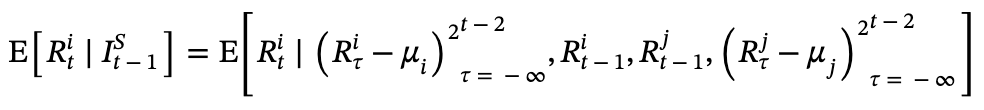
\includegraphics{granger_causality_1.png}
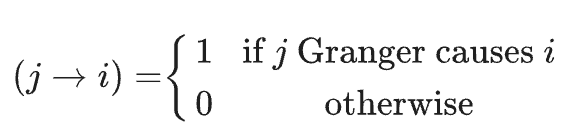
\includegraphics{granger_causality_2.png}

In general, if country j causes volatility in country i, then they are connected from j to i in one direction. There is a possibility in which country i does not cause any volatility in country j, indicating the edge is only one way. Yujie Lai and Yibo Hu (2021) derived this formula to calculate the correlation of stock index volatility between two countries.

In another literature, Yuejiao et al. (2021) were proposing to analyze covid recession systemic risk using both leverage and correlation factors. They were using $\Delta$CoVaR to calculate the leverage for each bank in pre-covid and post-covid eras based on evolution of their asset over time. $\Delta$CoVaR is a metric to calculate the growth rate of the market value of assets and firstly introduced by Adrian and Brunnermeier (2016). As the market value of banks’ assets change over time, so does their leverage level in the interbank networks thus affecting their activities and might expose them to looming systemic risk. Yuejiao et al. (2021) derived the $\Delta$CoVaR equation based on the situation during covid outbreak and produce formula
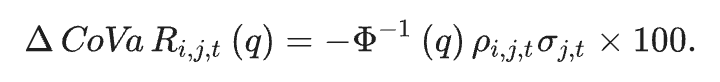
\includegraphics{covar.png}

This formula indicates that higher value of $\Delta$CoVaR means higher systemic value for bank q. The literature was using banks as the node and also using Granger-causality proposed by Billio et al. (2012) to determine connection between two banks.

\subsection{Centrality}
\subsection{Connectivity}
\subsection{Community Detection}

\section{Summary \& Conclusion}
This section will contain the summary from multiple approaches for systemic risk analysis in stock market

\section{Future Work}
This section will contain the potential future work for systemic risk analysis in stock market

%                Now build the reference list
\bibliographystyle{unsrt}   % The reference style
%                This is plain and unsorted, so in the order
%                they appear in the document.


\small
\bibliography{main}       % bib file(s).

\end{document}

